\problemname{Pixel Problem}

Simon thinks images are nice. He collects all kinds of images:
beautiful algorithmically generated images, northern Swedish landscapes, and screenshots of
various obscure mathematical proofs, to name a few. These are far from
all the categories of images that Simon has in his collection.

Now things have gone seriously wrong. Simon's hard drive has broken.
Fortunately, he managed to recover some of the images, but only the color data. In
other words, he has \emph{no idea} what dimensions the images had. And
on top of that, it also seems like Simon may not have managed to
recover all the pixels in the images. The only thing Simon is sure of is that at least one
pixel on the last row of each image remains, and all remaining pixels on the last row
are contiguous. The last row may \emph{thus} have been clipped
at some position.

\begin{figure}[ht!]
\centering
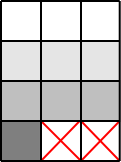
\includegraphics[width=0.2\textwidth]{example.png}
\caption{Miniature example of how an image can look after Simon's hard drive crash. The input
for this image would consist of 10 pixels in the list (two have been lost), and the white
pixels would come first, then the gray ones, etc. By looking at the image's pixels one can
conclude that the original width was probably 3 pixels.}
\label{fig:sample1}
\end{figure}

Now Simon needs expert help to determine the images' dimensions from
the color data and the information above. In his desperation, Simon goes to the
well-known Internet search engine Lolgee and searches for \texttt{"algorithm experts"}.
The first result is of course the \emph{Programming Olympiad}. It is your task
to help Simon as best you can.

\section*{Input}
Each test case contains exactly one image.

The first line contains an integer $N$ ($100 \leq N \leq 250\,000$), the number of pixels whose
color values Simon managed to recover. You thus know that the image contained at least
$N$ pixels (and possibly exactly $N$ pixels), but you do not know how many pixels
have disappeared from the last row of the image. You also know that the original width of
the image was at least $20$ pixels, and likewise the original height.

Then follows a line with $3N$ integers, a list of RGB values for each pixel.
The pixels are given in the order they are stored in Simon's computer, i.e. in \emph{row-major
order} (see Figure~\ref{fig:sample1}). The values for each pixel are given in the order \emph{red,
green, blue}. Each value is an integer between $0$ and $255$.

You can read more about the RGB color model on Wikipedia: \url{http://en.wikipedia.org/wiki/RGB_color_model}

\section*{Output}
Output a single integer: the original width of the image.

\section*{Examples}
There are a number of example images, with associated input and output that you
can download as a zip file from attachments.

``sample0x.in'' contains the image's color data, as described above (with the last row clipped).
``sample0x.ans'' contains the answer, i.e. the original width of the image.
``sample0x.png/jpg'' is the original image, in PNG or JPEG format.

\section*{Scoring}
Your program will be tested on 25 images and receives 4 points for each correct answer.
